\documentclass{beamer}
\usetheme{Madrid}
\usepackage{pgfplots}
\pgfplotsset{compat=1.15}
\usepackage{mathrsfs}
\usetikzlibrary{arrows}
\usepackage[utf8]{inputenc}
\usepackage{xcolor}
\usepackage{nicematrix}
\usepackage{tikz}
\usepackage{comment}
\usepackage{hyperref}
\usepackage{fancyvrb}
\usepackage{mathtools}
\usepackage{comment}
\usepackage{array}
\usepackage{bm}
\usepackage{pgfcore}
\usepackage{listings}
\usepackage{color}
\definecolor{munsell}{rgb}{0.0, 0.5, 0.69}
\definecolor{dkgreen}{rgb}{0,0.6,0}
\definecolor{gray}{rgb}{0.5,0.5,0.5}
\definecolor{mauve}{rgb}{0.58,0,0.82}
\definecolor{minas}{RGB}{0.244, 0.172, 0.36}
\definecolor{PUJ}{RGB}{44, 86, 151}
\definecolor{PUJ2}{RGB}{43, 93, 156}
\definecolor{PUJ3}{RGB}{20, 52, 107}
\definecolor{cyandk}{rgb}{0.0, 0.72, 0.92}
\setbeamerfont{frametitle}{size=\LARGE ,series=\bfseries}
\setbeamercolor{frametitle}{fg=black, bg=white} %% title of the beamer
\setbeamercolor{titlelike}
{parent=structure,bg=PUJ2}
\setbeamercolor{title}{fg=white, bg=black} 
%\setbeamercolor{navigation symbols}{fg=white, bg=white}
\setbeamercolor*{palette primary}{use=structure,fg=black,bg=yellow}
\setbeamercolor*{palette secondary}{use=structure,fg=white,bg=black}
\setbeamercolor*{palette tertiary}{use=structure,fg=white,bg=black}

\setbeamercolor{block title}{bg=black,fg=white}


%% code information
\lstset{frame=tb,
  language=Python,
  aboveskip=3mm,
  belowskip=3mm,
  showstringspaces=false,
  columns=flexible,
  basicstyle={\small\ttfamily},
  numbers=none,
  classoffset=1,
  morekeywords={True,False}, keywordstyle=\color{munsell}, 
  classoffset=0, 
  keywordstyle=\color{blue},  
  commentstyle=\color{dkgreen},
  stringstyle=\color{PUJ3},
  numberstyle=\tiny\color{gray},
  breaklines=true,
  breakatwhitespace=true,
  tabsize=4,
}

%% You can change default language in the middle of document with \lstset{language=Java}.


%% PUT or Remove the logo in a slide.


%% Information topic

\institute{BIT}
\date{2020}

\title[BIT] %optional
{Determinantes de la educación }
\subtitle{}

\author[Daniela \& Juan] 
{
La daniela y el juan}

\institute[] 
{
  BIT\\
  \and
  
\textbf{carlos@gmail.com}
}

\date[BIT] % (optional)

\newif\ifplacelogo % create a new conditional
\placelogotrue % set it to true
%\logo{\ifplacelogo\color{red}\rule{.5cm}{.5cm}\fi}
\logo{\ifplacelogo \includegraphics[height= 1cm]{BIT.eps}\fi}



\begin{document}



\frame{\titlepage}


\begin{frame}
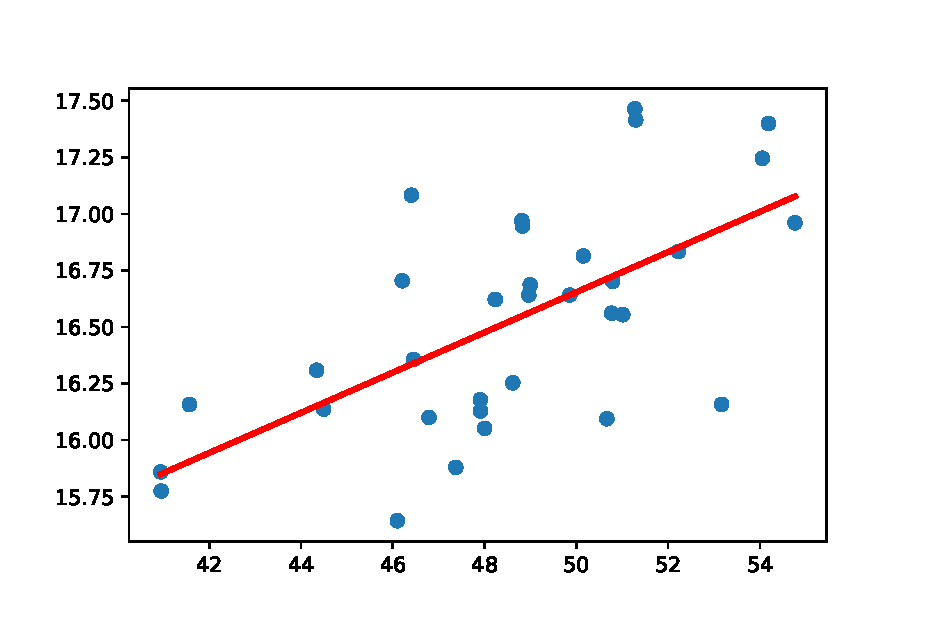
\includegraphics[scale=0.5]{intro.eps}
\end{frame}


\begin{frame}{Introducción}
La mortalidad materna es un indicador multidimensional.
\end{frame}

\begin{frame}{Justificación}
Es un objetivo del milenio por tanto monitorearlo es vital.
\end{frame}

\begin{frame}{Objetivos}
Es un objetivo del milenio por tanto monitorearlo es vital.
\end{frame}

\begin{frame}{Metodología}{Modelo}
\begin{equation}
math_{i} = \beta_{0} + \beta_{1}Sexo_{i} + \beta_{2}Edad_{i} + \beta_{3}Profesores_{i}
\end{equation}
\end{frame}

\begin{frame}{Metodología}{MCO}
\begin{equation}
\bm{\hat
{u}^{t}}\bm{\hat{u}} = 
\bm{y^{t}y - 2\hat{\beta}^{t} X^{t}y + \beta^{t}X^{t}X\beta}
\end{equation}
La forma matricial de $\sum u_{i}^{2} = (y_{i} - \hat{y_{i}})^{2}$.
La elección del vector de $\bm{\beta}$ que minimize el error, así:
\begin{equation}
\frac{\partial \bm{\hat
{u}^{t} \hat{u}} }{\partial \bm{\beta}}=0
\end{equation}
\begin{equation}
\bm{\beta^{*}}=
\bm{(X^{t}X)^{-1}X^{t}y}
\end{equation}
\end{frame}


\end{document}